\chapter{Sample Selections and Systematics}
\label{chap:SelsAndSysts}

\section{Systematic Uncertainties}
\label{sec:SelsAndSysts_Systs}

The systematics for this uncertainty are split into the groups, or blocks, depending on their purpose. They consist of flux uncertainties, neutrino-matter interaction systematics and detector efficiencies. There are also uncertainties on the oscillation parameters which this analysis will not be sensitive to, \delmsqsol and \sinsqsol. As described in \autoref{chap:MarkovChainMonteCarlo}, each model parameter used within this analysis requires a prior uncertainty. This is provided via separate covariance matrices for each block. The covariance matrices can include prior correlations between parameters within a single block, but the separate treatment means prior uncertainties can not be included for parameters in different groups. Alternatively, some parameters have no reasonably motivated uncertanities. These parameters are assigned flat priors which do not change the likelihood penalty. The flux, neutrino interaction and detector modelling has already been discussed in \autoref{sec:Simulations_Simulation}. The uncertainties invoked within these models are described below.

\subsection{Beam Flux}
\label{sec:SelsAndSysts_Systs_BeamFlux}

The neutrino beam flux systematics are based upon our uncertainty in the modelling of the components of the beam. This includes: the hadron production model and their re-interactions, the shape, intensity and alignment of the beam with respect to the target, and the uniformity of the magnetic field produced by the horn, alongside other effects. The uncertainty, as a function of neutrino energy, is illustrated in \autoref{fig:SelsAndSysts_BeamFluxSysts} which includes the total uncertainty as well as the individual components. The uncertainty for events below, and much higher than, the peak neutrino energy is dominated by hadron production and re-interaction systematics. The beam profile and alignment of the proton beam dominates the systematic uncertainty for events with \quickmath{E_{\nu} \sim 1\text{GeV}}. 

\begin{figure}[h]
  \begin{subfigure}[t]{\textwidth}
    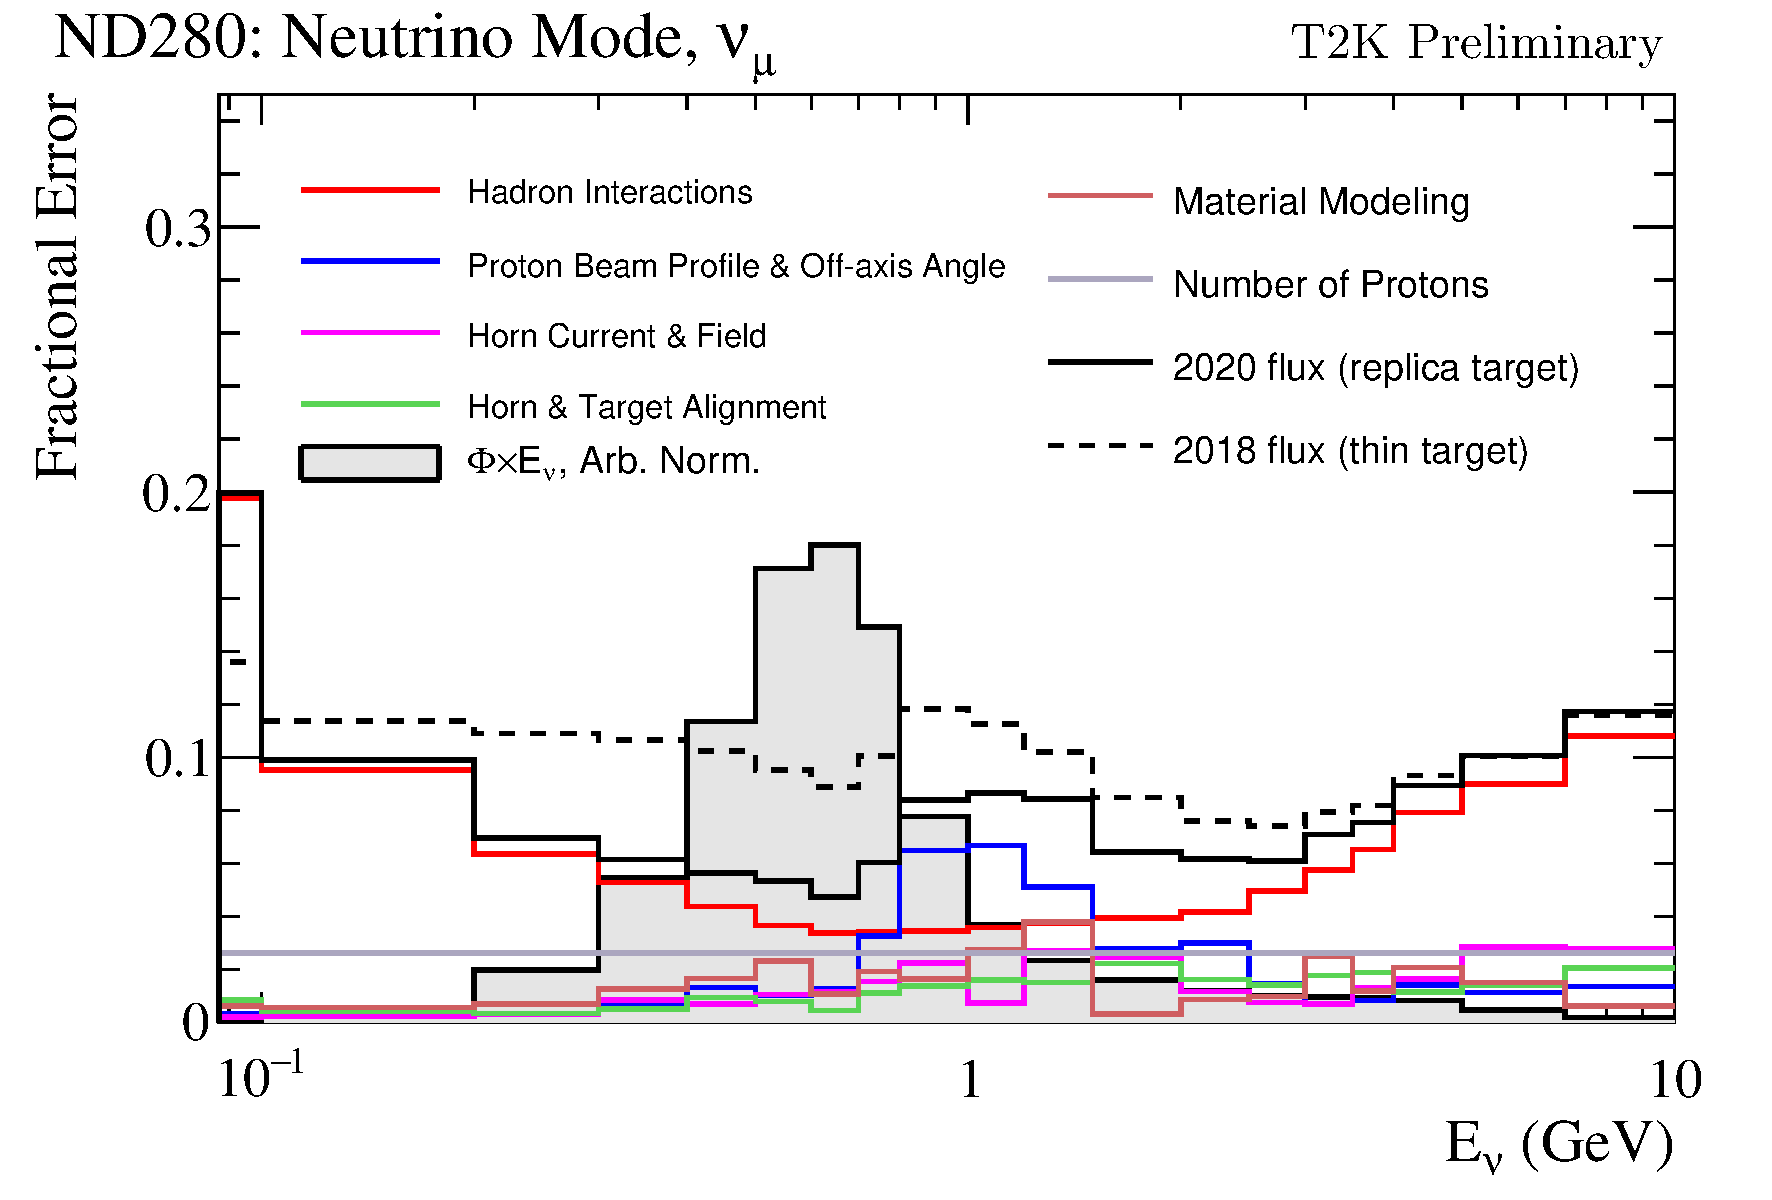
\includegraphics[width=\textwidth, trim={0mm 0mm 0mm 0mm}, clip,page=1]{Figures/Selections/flux_uncertainty_covariance_plots_addcorrnd_compwv3_flux_error_t2k_nd5_fhc_numu.pdf}
  \end{subfigure}
  %\begin{subfigure}[t]{\textwidth}
  %  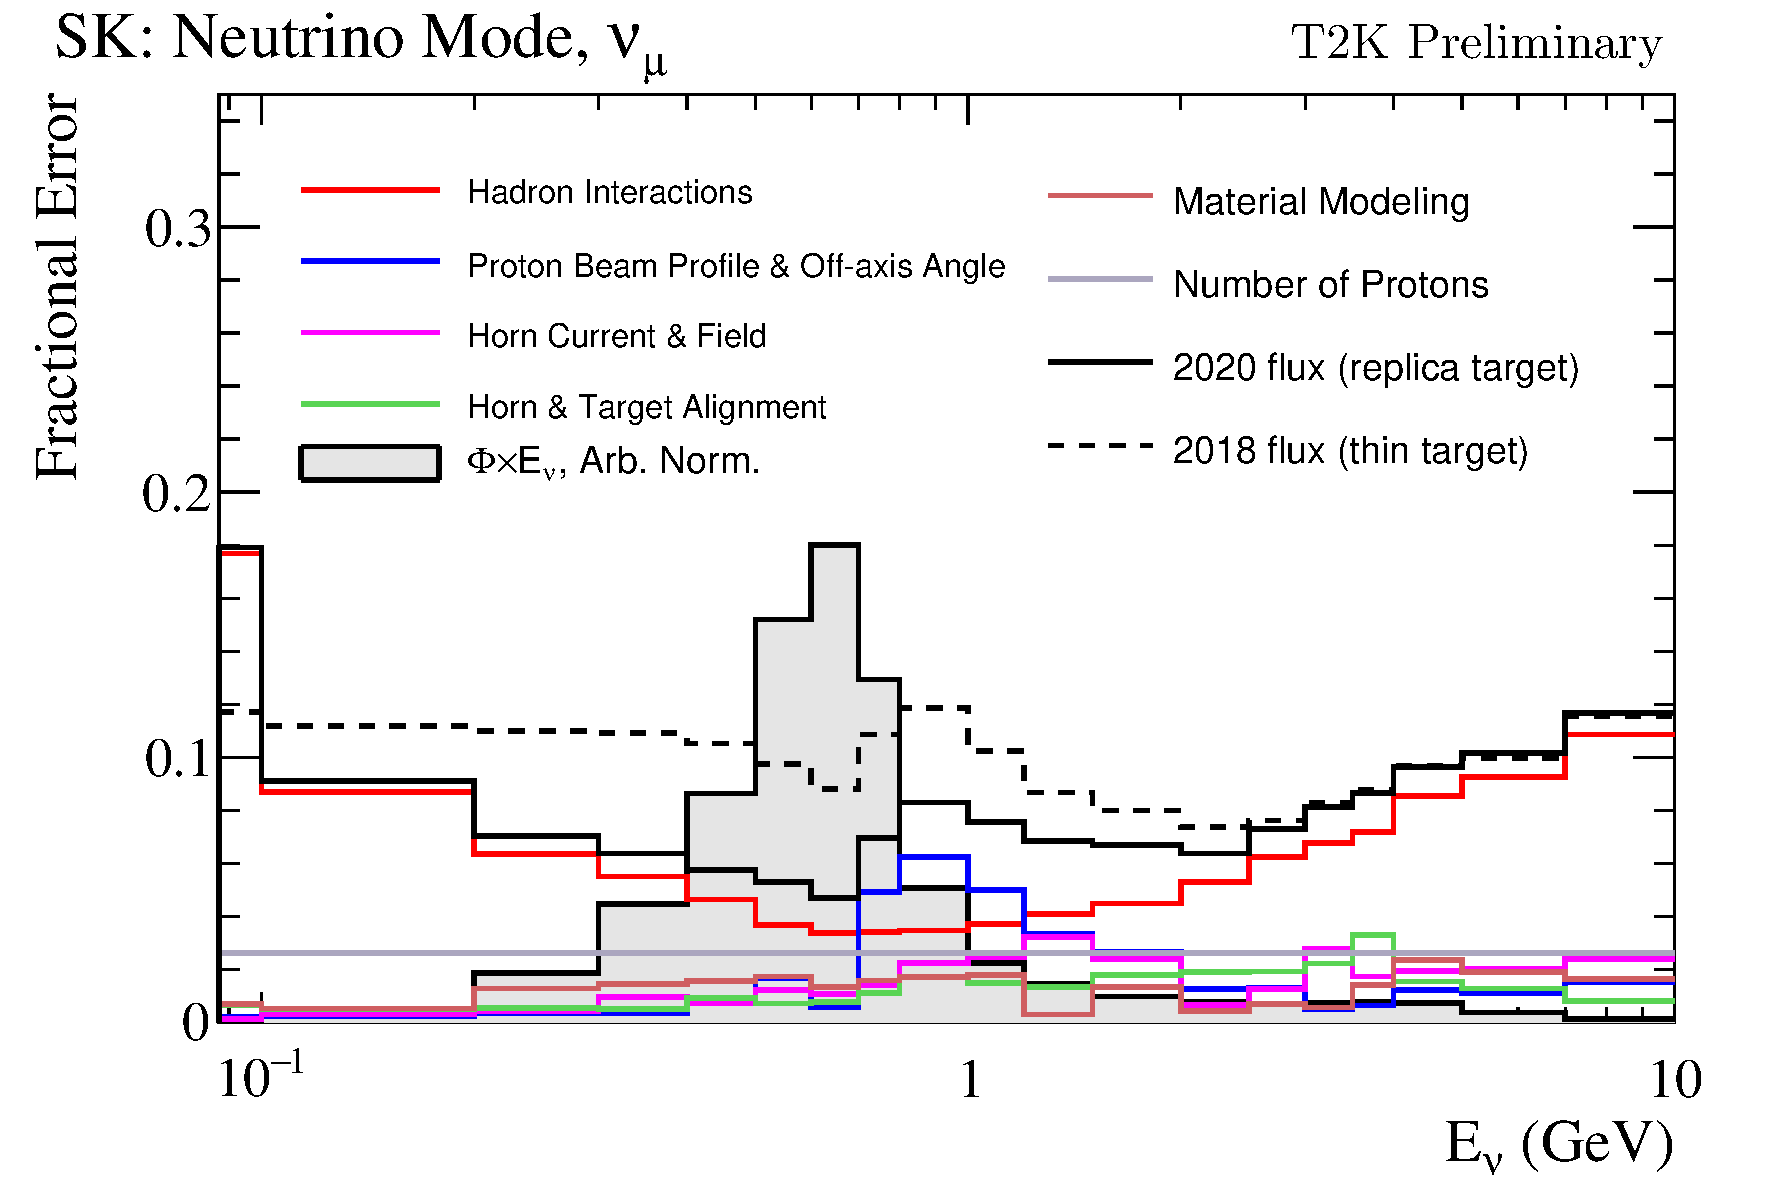
\includegraphics[width=\textwidth, trim={0mm 0mm 0mm 0mm}, clip,page=1]{Figures/Selections/flux_uncertainty_covariance_plots_addcorrnd_compwv3_flux_error_t2k_sk_fhc_numu.pdf}
  %\end{subfigure}
  \caption{The total uncertainty evaluated on the near detector \quickmath{\nu_{\mu}} flux prediction constrained by the replica-target data, illustrated as a function of neutrino energy. The solid(dashed) line indicates the uncertainty used within this analysis(the T2K 2018 analysis). The solid histogram indicates the neutrino flux as a function of energy. Figure taken from \cite{t2k_tn_354}.}
  \label{fig:SelsAndSysts_BeamFluxSysts}
\end{figure}

The beam flux uncertainties are described by one hundred parameters. They are split between both ND280 and SK detectors and binned by neutrino flavour: \quickmath{\nu_{\mu}}, \quickmath{\bar{\nu}_{\mu}}, \quickmath{\nu_{e}} and \quickmath{\bar{\nu}_{e}}. The response is then broken down as a function of neutrino energy. The bin density in the neutrino energy is the same for the FHC-\quickmath{\nu_{\mu}} and RHC-\quickmath{\bar{\nu}_{\mu}}, and narrows for neutrino energies close to the oscillation maxima of \quickmath{E_{\nu} = 0.6\text{GeV}}. This binning is specified in \autoref{tab:SelsAndSysts_BeamFluxBinEdges}. All of these systematic uncertanties are applied as normalisation parameters with Gaussian priors centered at \quickmath{1.0} and error specified from a covariance matrix provided by the T2K beam group.

\begin{table}[ht!]
    \centering
    \begin{tabular}{c|c|c}
      \hline
      Neutrino Flavour & Sign & Neutrino Energy Bin Edges (GeV) \\
      \hline
      \quickmath{\mu} & Right & \quickmath{0.,0.4,0.5,0.6,0.7,1.,1.5,2.5,3.5,5.,7.,30.} \\
      \quickmath{\mu} & Wrong & \quickmath{0.,0.7,1.,1.5,2.5,30.} \\
      \quickmath{e} & Right & \quickmath{0.,0.5,0.7,0.8,1.5,2.5,4.,30.} \\
      \quickmath{e} & Wrong & \quickmath{0.,2.5,30.} \\
      \hline
      \hline
    \end{tabular}
    \caption{The neutrino energy binning for the different neutrino flavours. ``Right'' sign indicates neutrinos in the FHC beam and antineutrinos in the RHC beam mode. ``Wrong'' sign indicates antineutrinos in the FHC beam and neutrinos in the RHC beam mode. The binning of the detector response is identical for the FHC and RHC modes as well as at ND280 and SK.}
    \label{tab:SelsAndSysts_BeamFluxBinEdges}
\end{table}

\subsection{Atmospheric Flux}
\label{sec:SelsAndSysts_Systs_AtmFlux}
The atmospheric neutrnio flux is modelled by the HKKM model, however 16 systematic uncertainties are applied to control the normalisation of each neutrino flavour, energy and direction. All of the parameters are given Gaussian priors centered at \quickmath{0} and width \quickmath{1.}. They are summarised below:

\begin{itemize}
\item \textbf{Absolute Normalisation}: The overall normalisation of each neutrino flavour is controlled by two indpendent systematic uncertainties, for \quickmath{E_{\nu} < 1\text{GeV}} and \quickmath{E_{\nu} > 1\text{GeV}}, respectively. This is driven mostly by hadronic interaction uncertainties for the production of pions and kaons \cite{Honda_2007}. The strength of the response is dependent upon the neutrino energy.
\item \textbf{Relative Normalisation}: Uncertainties on the ratio of \quickmath{(\nu_{\mu} + \bar{\nu}_{\mu})/(\nu_{e} + \bar{\nu}_{e})} are controlled by the difference between the HKKM model \cite{Honda_2007}, FLUKA \cite{etde_20239111} and Bartol models \cite{Barr_2004}. Three independent parameters are applied in the energy ranges: \quickmath{E_{\nu} < 1\text{GeV}}, \quickmath{1\text{GeV} < E_{\nu} < 10 \text{GeV}}, and \quickmath{E_{\nu} > 10\text{GeV}}.
\item \textbf{\quickmath{\nu}/\quickmath{\bar{\nu}} Normalisation}: The uncertainties in the \quickmath{\pi^{+}/\pi^{-}} (and kaon equivalent) produce uncertainties in the flux of \quickmath{\nu/\bar{\nu}}. The response is applied in the same way as the relative normalisation parameters.
\item \textbf{Up/Down and Vertical/Horizontal Ratio}: Similar to the above two systematics, the difference between the HKKM, FLUKA and Bartol model predictions, as a function of \quickmath{\cos(\theta_{Z})}, is used to control the normalisation of events as a function of zenith angle.
\item{\textbf{\quickmath{K/\pi} Ratio}}: Higher energy neutrinos (\quickmath{E_{\nu} < 10\text{GeV}}) become dependent upon kaon decay as the dominant source of neutrinos. Measurements of the ratio of \quickmath{K/\pi} \cite{Ambrosini1998-er} are used to control the systematic uncertainty of the expected ratio of pion and kaon production.
\item \textbf{Solar Activity}: As the 11-year solar cycle can affect the Earth's magnetic field, the flux of primary cosmic rays is modulated across the same period. The uncertainity is calculated by taking a \quickmath{\pm 1} year variation, equating to a \quickmath{10\%} uncertainty for the SK-IV period.
\item \textbf{Atmospheric Density}: The height of the interaction of the primary cosmic rays is dependent upon the atmospheric density. The HKKM assumes the US standard 1976 \cite{USStandardAtm} profile. This systematic controls the uncertainty in that model.
\end{itemize}

Updates to the HKKM and Bartol models are underway to use a similar tuning technique to that used in the beam flux predictions. After those updates, it may be possible to include correlations in the hadron production uncertanty systematics for beam and atmospheric flux predictions.

\subsection{Neutrino Interaction}
\label{sec:SelsAndSysts_Systs_Interaction}

